%%%%%%%%%%%%%%%%%%%%%%%%%%%%%%%%%%%%%%%%%%%%%%%%%%%%%%%%%%%%%%%%%%%%%%%%
% Plantilla TFG/TFM
% Escuela Politécnica Superior de la Universidad de Alicante
% Realizado por: Jose Manuel Requena Plens
% Contacto: info@jmrplens.com / Telegram:@jmrplens
%%%%%%%%%%%%%%%%%%%%%%%%%%%%%%%%%%%%%%%%%%%%%%%%%%%%%%%%%%%%%%%%%%%%%%%%

\chapter{Resultados}

En este capítulo se presentan los resultados finales obtenidos tras la implementación y validación del sistema de monitorización de red desarrollado. A diferencia del capítulo anterior, centrado en la verificación funcional del sistema, en este apartado se describen las pantallas finales de la aplicación desde el punto de vista del ususario, destacando la información proporcionada y su utilidad para la monitorización y gestión de la red.

Las vistas mostradas corresponden corresponden al estado final del sistema y reflejan el funcionamiento normal de la aplicación una vez superadas las pruebas descritas previamente.

\section{Vista de estado del router}

La vista de estado del router proporciona una visión general del funcionamiento del dispositivo seleccionado, permitiendo al usuario conocer de forma inmediata su situación operativa. En esta pantalla se muestran parámetros relevantes como el \textit{uptime}, la versión del sistema operativo, el modelo del dispositivo y el uso de recursos, como la carga de la CPU.

Esta información resulta especialmente útil para detectar posibles problemas de rendimiento o identificar routers que puedan requerir una intervención preventiva. La Figura~\ref{fig:resultado-estado-router} muestra un ejemplo de esta vista, donde se aprecia la información consolidada del router seleccionado.

\begin{figure}[H]
  \centering
  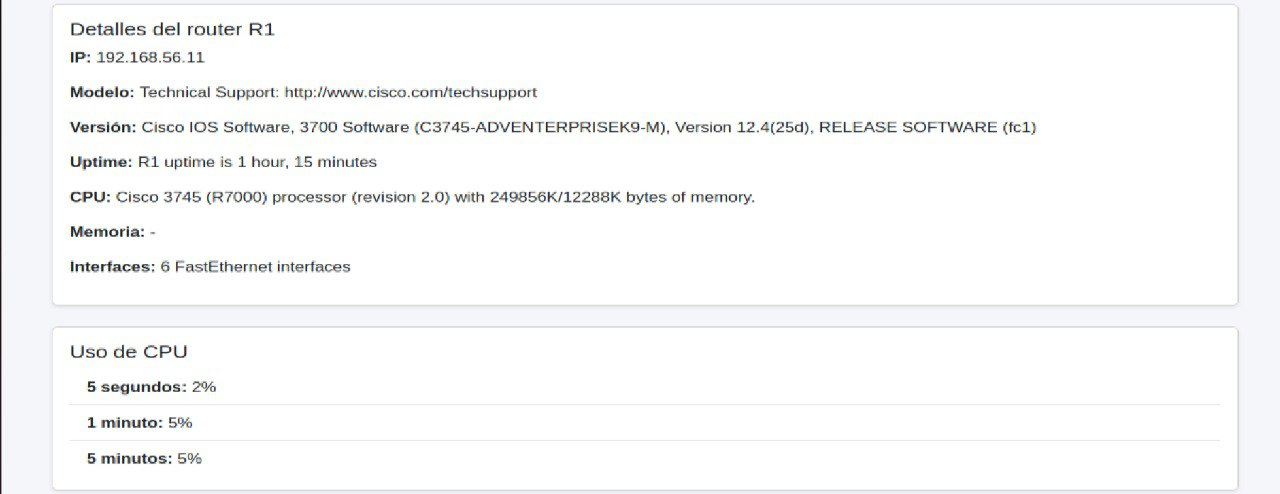
\includegraphics[width=\textwidth]{imagenes/Estado del Router_dos.jpg}
  \caption{Vista final del estado del router con información general y uso de recursos.}
  \label{fig:resultado-estado-router}
\end{figure}

\section{Vista de interfaces de red}

La vista de interfaces de red constituye uno de los elementos principales del sistema de monitorización, ya que permite analizar de forma detallada el estado de cada interfaz del router. En esta pantalla se muestran datos como la dirección IP, el estado administrativo, el estado del protocolo, la velocidad, el modo dúplex y la existencia de errores.

La representación visual empleada facilita la identificación rápida de incidencias, permitiendo al usuario detectar interfaces con problemas de forma inmediata. Además, desde la vista es posible realizar acciones de gestión sobre las interfaces, lo que conivierte a esta pantalla en una herramienta práctica para la administración de la red. La Figura~\ref{fig:resultado-interfaces} muestra la vista final de interfaces implementada en el sistema.

\begin{figure}[H]
  \centering
  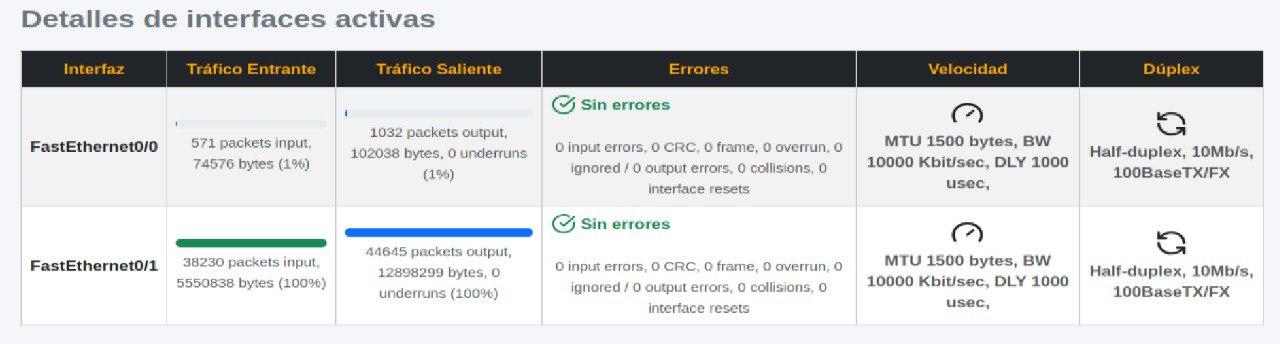
\includegraphics[width=\textwidth]{imagenes/Interfaces de Red_dos.jpg}
  \caption{Vista final de monitorización y gestión de interfaces de red.}
  \label{fig:resultado-interfaces}
\end{figure}

\section{Visualización del tráfico de red}

El sistema incorpora representaciones gráficas que permiten analizar el táfico de red de manera intuitiva. estas gráficas muestran el tráfico entrante y saliente de las interfaces, facilitando la comparación entre distintos enlaces y la detección de positbles desequilibrios o sobrecargas.

La visualización gráfica complementa la información numérica y aporta una interpretación más clara del comportamiento de la red, especialmente en escenarios donde se requiere un análissis rápido del flujo de datos. EN la Figura~\ref{fig:resultado-trafico} pse presenta un ejemplo de las gráficas de tráfico generadas por el sistema.

\begin{figure}[H]
  \centering
  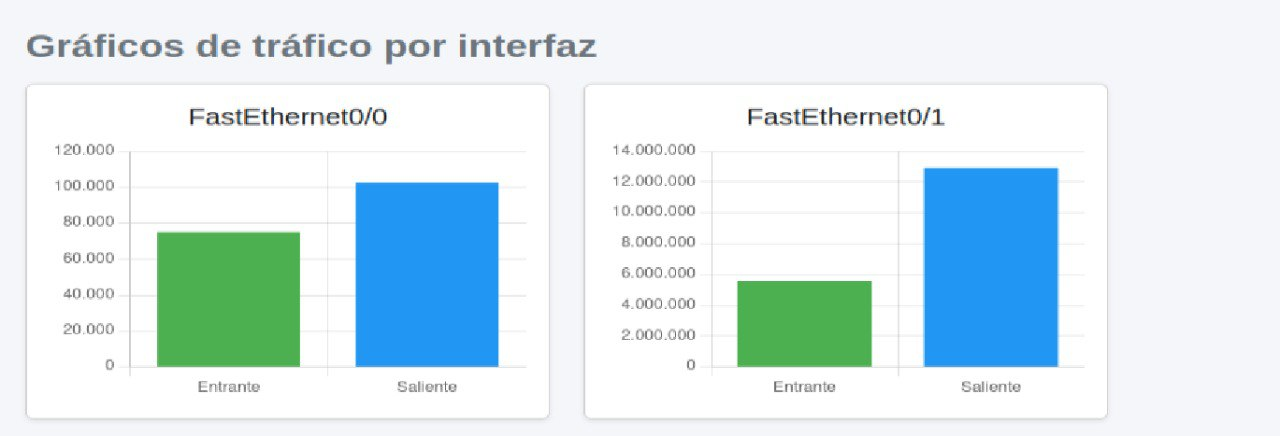
\includegraphics[width=\textwidth]{imagenes/Interfaces de Red_tres.jpg}
  \caption{Visualización gráfica del tráfico entrante y saliente por interfaz.}
  \label{fig:resultado-trafico}
\end{figure}

\section{Sistema de alertas e informes}

Como resultado adicional del sistema desarrollado, se disponte de un mecanismo de alertas que notifica al usuasrio cuando se detectan errores en las interfaces de red. Este sistema genera automáticamente un informe en formato PDF con el resumen de las incidencias detectadas y lo envía por correo electrónico al usuario autenticado.

Este enfoque permite una supervisión proactiva de la red, ya que el administrados puede ser informado de problemas relevantes sin necesidad de acceder continuamente a la aplicación web. La integración de este sistema de alertas incrementa el valor práctico de la herramienta y la acerca al funcionamiento de soluciones profesionales de monitorización.

\section{Valoración global de los resultados}

Los resultados obtenidos demuestran que el sistema desarrollado cumple con los objetivos planteados al inicio del trabajo, proporcionando una solución funcional para la monitorización y gestión básica de una red de comunicaciones. Las distintas vistas implementadas permiten al usuario obtener información relevante de forma clar y estructurada, facilitando la toma de decisiones y la detección temprana de incidencias.

El conjunto de funcionalidades presentadas constituye una base sólida sobre la que se pueden incorporar mejoras futuras, como el almacenamiento histórico de datos, la ampliación del sistema de alertas o la integración de nuevos dispositivos de red, aspectos que se abordan en el capítulo de conclusiones y trabajos futuros.


